\chapter{Design \& Deployment of MIBot for Human Feasibility Study}
\label{ch:mibot}

The recent advances in Large Language Models (LLMs) present an opportunity to automate various forms of mental health talk therapy, including Motivational Interviewing (MI) for smoking cessation. This is a significant area of need, as over half of all smokers are in an ambivalent state, where they are aware of the harms of smoking but have not yet committed to quitting \citep{Babb2017}. Guiding these individuals towards a decision to quit is a key precursor for any successful quit attempt \citep{West2006}.

This chapter details the design and deployment of \margindex{MIBot}MIBot. It is a \margindex[MIBot]{fully generative}[Generative] LLM-based MI chatbot created for this purpose. The work builds on a predecessor system, MIBot v5.2 \citep{info:doi/10.2196/49132}, which, being partially scripted, had limitations in conversational naturalness. The development and evaluation of the current MIBot system are described in detail by \citet{mahmood-etal-2025-fully}. This chapter complements that work by focusing on the technologies, design considerations, and implementation choices underlying the chatbot's deployment for a human feasibility study.

The chapter is structured as follows. Section~\ref{sec:iterative-development} outlines the clinician-informed, iterative process used to develop the chatbot's core prompt. Section~\ref{sec:observers} describes the system architecture, including the observer agents designed to ensure safety and conversational coherence. Section~\ref{sec:deployment} details the technical implementation and deployment of the MIBot service using containerization and cloud infrastructure. Finally, Section~\ref{sec:feasibility} describes the design of the human feasibility study used to evaluate MIBot's effectiveness, focusing on four key dimensions: changes in participants' readiness to quit, perceived empathy (CARE scale), the chatbot's adherence to MI principles (AutoMISC), and its ability to elicit client change talk. Chapter~\ref{ch:mibot-eval} reports the results of this study.




\section{Chatbot Design Process}
\label{sec:iterative-development}

The design of MIBot followed a \margindex[MIBot]{clinician-informed}[Clinician-Informed] design process. This was an \margindex[MIBot]{iterative process}[Iterative] that combined expertise in MI with prompt engineering for a state-of-the-art LLM \cite{openai2024gpt4ocard}.

\subsection{Single-Prompt Architecture Rationale}
\label{sec:single-prompt-rationale}

The initial architectural decision for MIBot was to use a \margindex[MIBot]{single-prompt architecture}[Single-Prompt Arch.]single, comprehensive prompt to define the chatbot's behaviour. This ``start simple'' approach is a fundamental engineering principle, where the goal is to first build and test the most straightforward solution before considering more complex alternatives. In the context of an MI chatbot, a single prompt that encapsulates the counsellor's entire persona, skills, and decision-making logic provides a strong baseline for evaluation. If this simple architecture can be shown to be effective, it avoids the premature introduction of more complex systems, such as those involving multiple, dynamically selected prompts or a separate "Behavior-Change" selector module. The iterative development process described in the following section was therefore focused on refining this single prompt to its maximum potential.

\subsection{Iterative Prompt Development}
The MIBot prompt was refined through structured feedback from both engineers and experienced MI clinicians who regularly met biweekly over the course of development. The process began with a minimal prompt that instructed the model to act as an MI counsellor. This baseline was tested through simulated counselling sessions with two types of test clients:

\begin{enumerate}
    \item \textbf{\margindex[MIBot]{virtual smoker clients}[Virtual Smokers]Virtual smoker clients}, which were separate GPT-4o instances that were given detailed backstories and instructed to role-play smokers with varying attitudes toward quitting. Chapter~\ref{ch:synthetic-smoker} describes in detail the creation of these basic LLM-based virtual smokers, and subsequent research to enhance their capabilities.
    \item \textbf{\margindex[MIBot]{human role-playing}[Human Role-Play]Human role-playing as smokers} --- members of our research team who adopted smoker personas and interacted with the chatbot to test how each version of the prompt behaved in different scenarios.
\end{enumerate}

After each testing cycle, transcripts were reviewed in bi-weekly meetings to identify shortcomings in the appropriate use of MI skills, adherence to MI principles, tone, pacing, and client engagement, among other aspects. These findings informed successive prompt revisions. 
This process led to several key prompt revisions:


\begin{enumerate}
    \item \textbf{\margindex[MIBot, Prompt]{utterance length control}[Length Control]Utterance Length Control.} Early versions tended toward long, paragraph-like responses, which risked dominating the conversation, which is the antithesis of MI, in which the client leads the process of contemplation.  The prompt was amended to include explicit length constraints (``Keep your responses short. Do not talk more than your client.'') and to encourage brevity while maintaining reflective depth.

    \item \textbf{\margindex[MIBot, Prompt]{accessible language}[Accessible Lang.]Accessible Language.} To ensure inclusivity across educational and socioeconomic backgrounds, clinicians requested avoidance of jargon and adaptation to the client's linguistic style. This was codified in the prompt as ``Avoid using complex terminology … maintain simplicity in the conversation.''

    \item \textbf{\margindex[MIBot, Prompt]{assumption avoidance}[No Assumptions]Avoidance of Assumptions.} The model occasionally assumed the client's nicotine consumption patterns. The prompt was revised to explicitly instruct the counsellor that ``You don't know anything about the client's nicotine use yet'' to preserve an open, exploratory stance.

    \item \textbf{\margindex[MIBot, Prompt]{rapport-building}[Rapport]Rapport-Building Before Smoking Focus.} Initial versions of the prompt engaged with smoking behaviour too early, bypassing engagement and focusing stages. The revised prompt added guidance to ``open the conversation with a general greeting and friendly interaction'' before gradually steering toward smoking ambivalence.

    \item \textbf{Guarding Against \margindex[MIBot, Prompt]{premature planning}[No Planning]Premature Planning.} Planning is an MI process best introduced after sufficient evocation of Change Talk. The prompt included multi-step criteria for initiating planning, explicitly instructing the model to wait for reduced Sustain Talk and to confirm readiness before launching into planning and discussing concrete steps to take towards quitting.

    
\end{enumerate}



This iterative process continued until virtual and role-played conversations consistently met MI quality expectations as determined by an informal consensus of the team.


Tables~\ref{tab:initial-system-prompt} and \ref{tab:final-system-prompt} showcase how the prompt evolved from a simple instruction about the LLM's role to a comprehensive guideline addressing issues identified in the chatbot's performance.

\setlist[enumerate]{leftmargin=*, itemsep=0pt, topsep=2pt, parsep=0pt, partopsep=0pt}

% ===== Table 1: Initial system prompt =====
\begin{table}
  \centering
  \renewcommand{\arraystretch}{1.12}
  \begin{tcolorbox}[breakable,
                    colback=magenta!5!blue!10,
                    colframe=magenta!60!blue!40,
                    fonttitle=\bfseries,
                    fontupper=\footnotesize,
                    label=sec:initial_system_prompt]
  \noindent % Prevents indentation before tabularx
  \begin{tabularx}{\linewidth}{r Y} % Right-align numbers, auto-expand text
  \centering
      \textbf{1} & You are a skilled motivational interviewing counsellor. \\
      \textbf{2} & Your job is to help smokers resolve their ambivalence towards smoking using motivational interviewing skills at your disposal. \\
      \textbf{3} & Your next client is \{client\_name\}. Start the conversation by greeting \{client\_name\}. \\
  \end{tabularx}
  \end{tcolorbox}
  \caption[Initial MIBot Prompt]{The initial system prompt used for MIBot. This version of the prompt is very simple and only instructs the model to act as an MI counsellor and greet the client.}
  \label{tab:initial-system-prompt}
\end{table}

% ===== Table 2: Final system prompt =====
\begin{table}
  \centering
  \renewcommand{\arraystretch}{1.12}
  \begin{tcolorbox}[breakable,
                    colback=magenta!5!blue!10,
                    colframe=magenta!60!blue!40,
                    fonttitle=\bfseries,
                    fontupper=\footnotesize,
                    label=sec:final_system_prompt]
  \noindent % Prevents indentation before tabularx
  \begin{tabularx}{\linewidth}{r Y} % Right-align numbers, auto-expand text
  \centering
  \textbf{1} & You are a skilled motivational interviewing counsellor. Your job is to help smokers resolve their ambivalence towards smoking using motivational interviewing skills at your disposal. Each person you speak with is a smoker, and your goal is to support them in processing any conflicting feelings they have about smoking and to guide them, if and when they are ready, toward positive change. \\


  \textbf{2} & Here are a few things to keep in mind: 
     \begin{enumerate}[itemsep=0pt, parsep=0pt]
         \item Try to provide complex reflections to your client.
         \item Do not try to provide advice without permission.
         \item Keep your responses short. Do not talk more than your client.
         \item Demonstrate empathy. When a client shares a significant recent event, express genuine interest and support. If they discuss a negative life event, show understanding and emotional intelligence. Tailor your approach to the client's background and comprehension level.
         \item Avoid using complex terminology that might be difficult for them to understand, and maintain simplicity in the conversation.
     \end{enumerate} \vspace{-\baselineskip} \\

  \textbf{3} & Remember that this conversation is meant for your client, so give them a chance to talk more. \\
  \textbf{4} & This is your first conversation with the client. Your assistant role is the counsellor, and the user's role is the client. \\
  \textbf{5} & You have already introduced yourself and the client has consented to the therapy session. \\
  \textbf{6} & You don't know anything about the client's nicotine use yet. \\
  \textbf{7} & Open the conversation with a general greeting and friendly interaction, and gradually lead the conversation towards helping the client explore ambivalence around smoking, using your skills in Motivational Interviewing. \\
  \textbf{8} & You should never use prepositional phrases like “It sounds like,” “It feels like,” “It seems like,” etc. \\
  \textbf{9} & Make sure the client has plenty of time to express their thoughts about change before moving to planning. Keep the pace slow and natural. Don't rush into planning too early. \\

  \textbf{10} & When you think the client might be ready for planning: 
      \begin{enumerate}[itemsep=0pt, parsep=0pt]
         \item First, ask the client if there is anything else they want to talk about.
         \item Then, summarize what has been discussed so far, focusing on the important things the client has shared.
         \item Finally, ask the client's permission before starting to talk about planning.
      \end{enumerate} \\

  \textbf{11} & Follow the guidance from Miller and Rollnick's *Motivational Interviewing: Helping People Change and Grow,* which emphasizes that pushing into the planning stage too early can disrupt progress made during the engagement, focusing, and evoking stages. \\

  \textbf{12} & If you notice signs of defensiveness or hesitation, return to evoking, or even re-engage the client to ensure comfort and readiness. \\

  \textbf{13} & Look for signs that the client might be ready for planning, like: 
      \begin{enumerate}[itemsep=0pt, parsep=0pt]
         \item An increase in change talk.
         \item Discussions about taking concrete steps toward change.
         \item A reduction in sustain talk (arguments for maintaining the status quo).
         \item Envisioning statements where the client considers what making a change would look like.
         \item Questions from the client about the change process or next steps.
      \end{enumerate} \\
  \end{tabularx}
  \end{tcolorbox}
    \caption[Final MIBot Prompt]{The final system prompt for MIBot, developed through an iterative, clinician-informed process. This version includes detailed instructions on MI skills, tone, pacing, and specific guidelines for handling different conversational stages, such as when to initiate planning.}
  \label{tab:final-system-prompt}
\end{table}


\begin{figure}[ht]
  \centering
  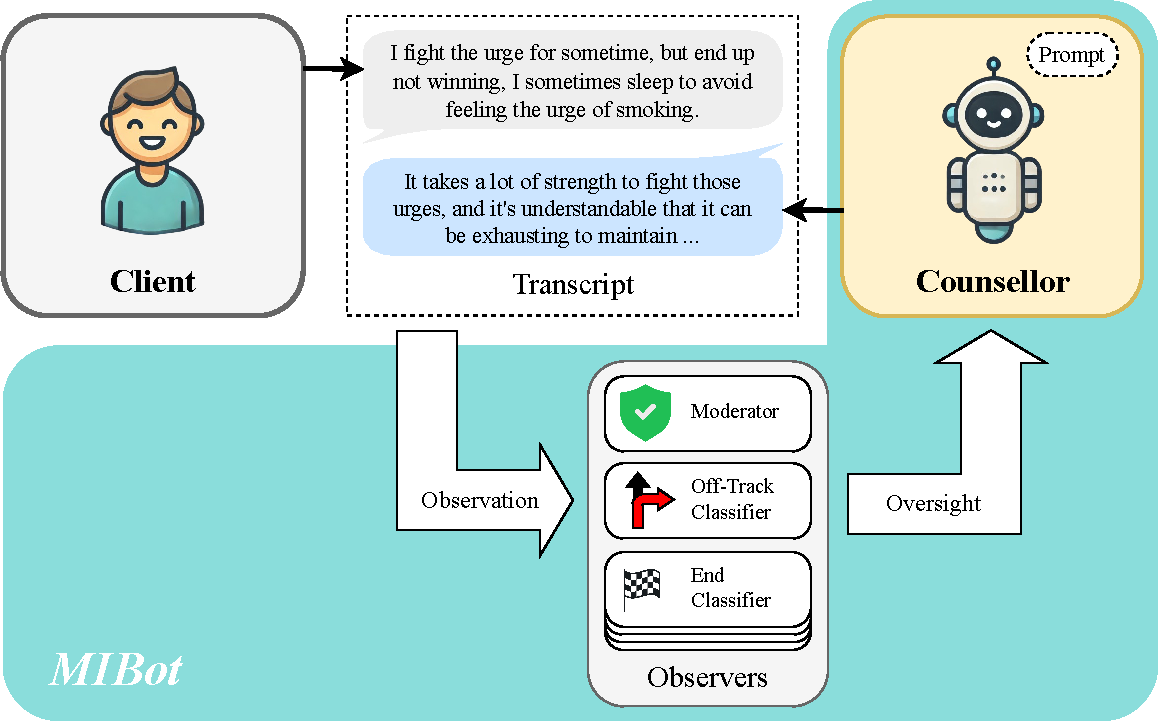
\includegraphics[width=0.9\linewidth]{fig/sysdiag.pdf} 
  \caption{Overview of the MIBot system, taken from \citet{mahmood-etal-2025-fully}}
  \label{fig:sysdiag}
\end{figure}

\section{Observers}
\label{sec:observers}
To enhance safety in the deployment of MIBot, the core counsellor agent was augmented with a set of \margindex[MIBot]{observer agents}[Observer Agents]\textit{observer agents}, independent instances of GPT-4o prompted to monitor specific aspects of the conversation in real time.  The output of these agents is used to intervene when necessary. Each observer was specialized through prompt engineering to perform a specific task in real time.

\subsection{Moderator}
The \margindex[MIBot, Observers]{moderator}[Moderator]\textit{Moderator} evaluates the counsellor's most recent utterance for potential harm before it is displayed to the client. While OpenAI's internal safety systems mitigate many risks, they do not address all possible counterproductive counselling behaviours, such as inadvertently reinforcing \emph{sustain talk} or suggesting self-harm. The Moderator was deliberately configured for high sensitivity, accepting a higher false positive rate to reduce the risk of harmful or counterproductive content. If a counsellor's utterance is flagged, it is regenerated and re-evaluated, with up to five regeneration attempts permitted. In all study conversations, an acceptable utterance was produced within four attempts, and no session failed to pass moderation.

\subsection{Off-Track Conversation Classifier}
The \margindex[MIBot, Observers]{off-track classifier}[Off-Track]\textit{Off-Track Classifier} detects when a client is steering the dialogue away from smoking cessation in a deliberate or sustained manner. Its prompt was tuned for low false positive rates to preserve conversational flexibility. In the feasibility study described in Chapter~\ref{ch:mibot-eval}, this observer's primary role was retrospective --- identifying conversations for exclusion where the participant was not engaging seriously with the intervention. In a live deployment, it can be a used to trigger early termination or redirection to the main topic.

\subsection{End Classifier \& Termination Process}
The \margindex[MIBot, Observers]{end classifier}[End Chat]\textit{End Classifier} monitors both parties' dialogue to determine if the conversation is reaching a natural conclusion. It prioritizes the client's intent when making this determination, ensuring the conversation is not ended prematurely. Upon detecting an intent to close, it instructs the counsellor to deliver a concise summary of key discussion points --- a standard MI practice --- and to confirm with the client whether they wish to continue. If the client declines, the conversation is terminated and any post-session procedures, such as surveys, are initiated.


\textbf{Design Rationale:} All observers were implemented as separate, stateless LLM calls, each with prompts tailored to their decision criteria. This modular approach allowed independent refinement of their sensitivity–specificity balance without impacting the primary counsellor prompt. The Moderator favoured recall over precision to err on the side of client safety, whereas the Off-Track Classifier did the opposite, favouring conversational autonomy. The End Classifier's logic explicitly distinguished between topic changes and true conversation endings, reducing false terminations.


The prompted GPT-4o, together with observers, constitute the complete MIBot system, as illustrated in Figure~\ref{fig:sysdiag}.


\section{MIBot System Design}
\label{sec:deployment}


\subsection{Overview of the Application}


MIBot is implemented as a containerized software system that can be run locally for development and deployed to cloud-based systems. In this section, we discuss the implementation details of MIBot, from the structure of the Python microservice and its integration with the OpenAI API to the containerization and the deployment of the service on Amazon Web Services.

At the heart of MIBot is a lightweight Python web application built with the \texttt{Sanic} framework \cite{pi_sanic}. In MIBot, \texttt{app.py} --- the main entry point --- uses \texttt{Sanic} to configure routes for all external interactions and instantiates the conversation engine.
\begin{figure}[ht]
  \centering
  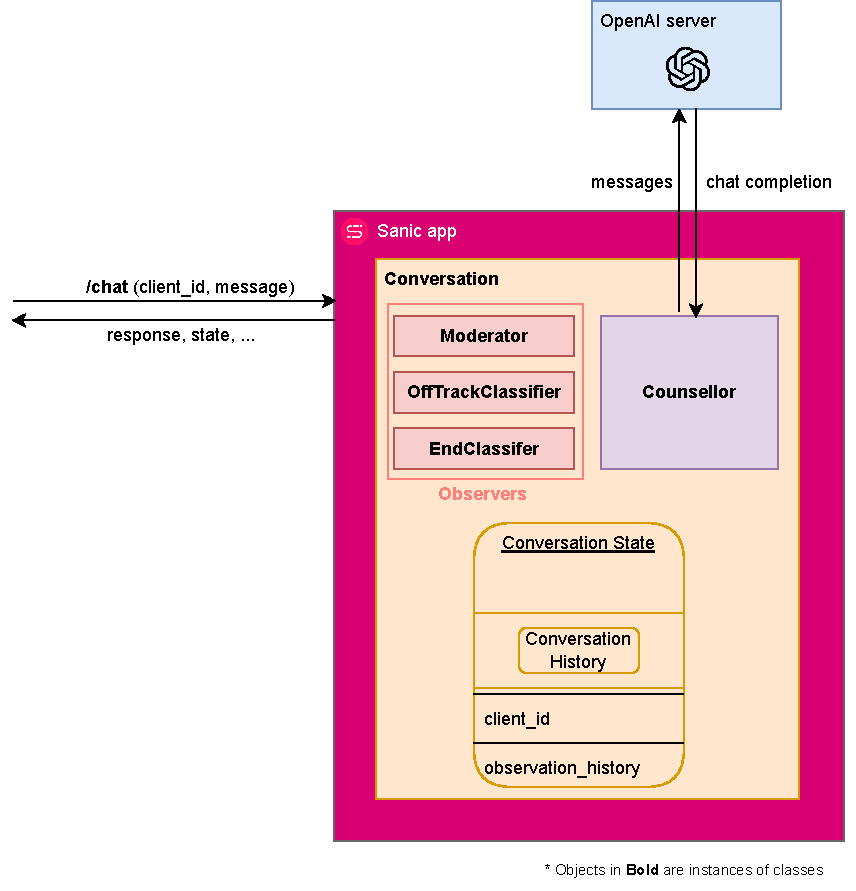
\includegraphics[width=0.7\linewidth]{fig/microservice.drawio.pdf} 
  \caption{Overview of the Sanic application that contains MIBot code and exposes REST APIs.}
  \label{fig:microservice}
\end{figure}
At the start of a conversation, the \texttt{Conversation} object is initialized, which creates and stores a list of \texttt{Observer} instances. It also creates a \texttt{Counsellor} object that encapsulates the chatbot logic (Figure~\ref{fig:microservice}). When a user sends a request to the \texttt{/chat} endpoint containing the client's message and \texttt{client\_id} in a structured JSON object, Sanic's route handler updates the state of the \texttt{Conversation} and requests the next turn from it. The \texttt{Conversation} object relays this to the \texttt{Counsellor}, which in turn sends a request to the OpenAI API with the accumulated conversation history and the current client message, and receives a \texttt{ChatCompletion} response. The \texttt{ChatCompletion} response contains the generated counsellor turn, which is returned to the \texttt{Conversation} object.

Each \texttt{Observer} attached to the \texttt{Conversation} inherits from a base class defining an asynchronous \texttt{observe()} method. As noted earlier, the \texttt{Moderation} observer screens counsellor utterances for safety and appropriateness; the \texttt{Offtrack} observer assesses whether the client is steering the conversation away from smoking cessation; and the \texttt{EndClassifier} determines when a session should conclude. These observers are implemented as separate GPT-4o API calls with their own prompts. After each turn, the \texttt{Conversation} object loops through all \texttt{Observer} objects, collects their observations, and makes real-time decisions (e.g., whether to end the conversation) before updating its state. If the generated output from the \texttt{Counsellor} is deemed suitable for the client, it is passed to Sanic's response handler, which packages it with metadata into a JSON object and sends it to the client.

A single \texttt{Sanic} app can handle multiple clients at once by creating replicas of the \texttt{Conversation} object, each uniquely identified by the \texttt{client\_id}.\footnote{For the human feasibility study, in order to keep track of the participants and their conversations, we explicitly use \texttt{prolific\_id} as \texttt{client\_id}. Prolific (\url{www.prolific.com}) is the platform we use to recruit participants and conduct our feasibility study. See Section~\ref{sec:feasibility-study} for further details.} The microservice also exposes some additional endpoints: \texttt{/get\_transcript} provides a downloadable transcript of the conversation for post-session analysis; \texttt{/health} returns a simple \texttt{200} response so that load balancers and orchestrators can perform health checks; and \texttt{/info} exposes build metadata such as the current version of the prompt.

\subsection{Containerization}

\begin{figure}[ht]
  \centering
  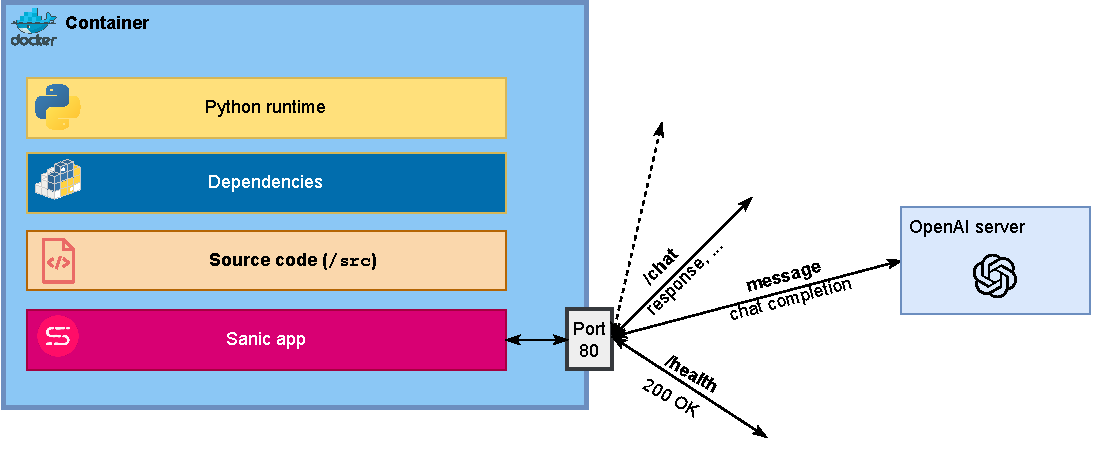
\includegraphics[width=0.7\linewidth]{fig/container.drawio.pdf} 
  \caption{Containerized Sanic application.}
  \label{fig:containerization}
\end{figure}

For reproducibility and ease of deployment, the microservice is packaged in a Docker container. Containerization provides several advantages for the development, testing, and deployment of MIBot:

\begin{itemize}
\item \textbf{Environment Consistency:} Containers encapsulate all dependencies, ensuring that the application behaves identically across local development machines, staging environments, and production servers. This eliminates the ``works on my machine'' problem.

\item \textbf{Portability:} The same container image can run on any system that supports Docker (or an OCI-compliant runtime), whether on a developer's laptop, an on-prem cluster, or a cloud provider like AWS, without modification.

\item \textbf{Isolation:} The application runs in its own isolated environment with a defined set of libraries and runtime parameters, preventing conflicts with other software on the host system.

\item \textbf{Scalability:} Container orchestration platforms such as Kubernetes or Amazon ECS can rapidly start and stop containers based on demand, enabling efficient horizontal scaling during high-traffic periods.

\item \textbf{Faster Deployment and Rollback:} Pre-built container \emph{images} can be deployed quickly, and previous versions can be rolled back by redeploying an earlier image tag, reducing downtime.

\item \textbf{Simplified CI/CD Integration:} Containers integrate seamlessly with continuous integration and delivery pipelines, allowing automated builds, tests, and deployments triggered by code changes.

\item \textbf{Reproducibility:} For experimental settings, distributing a container image ensures that collaborators can reproduce results exactly, regardless of local environment differences.
\end{itemize}

The MIBot container image is defined by a \texttt{Dockerfile} specifying the base Python runtime, required dependencies, the source code, and main entry point (\emph{viz.} \texttt{app.py}). This image is stored in Amazon Elastic Container Registry (ECR). The container registry stores all the images built by the CI/CD pipeline, but only the image with the \texttt{production} tag is used for deployment.

\section{Deploying MIBot to AWS}
\label{sec:mibot-deployment}

MIBot is deployed as a service on Amazon \textbf{Elastic Container Service (ECS)}. ECS is a fully managed service provided by Amazon Web Services (AWS) that ``simplifies the deployment, management, and scaling of applications using containers'' \cite{aws-ecs-getting-started}. We now discuss each component of ECS.

\subsection{Components of ECS}
\begin{figure}[ht]
  \centering
  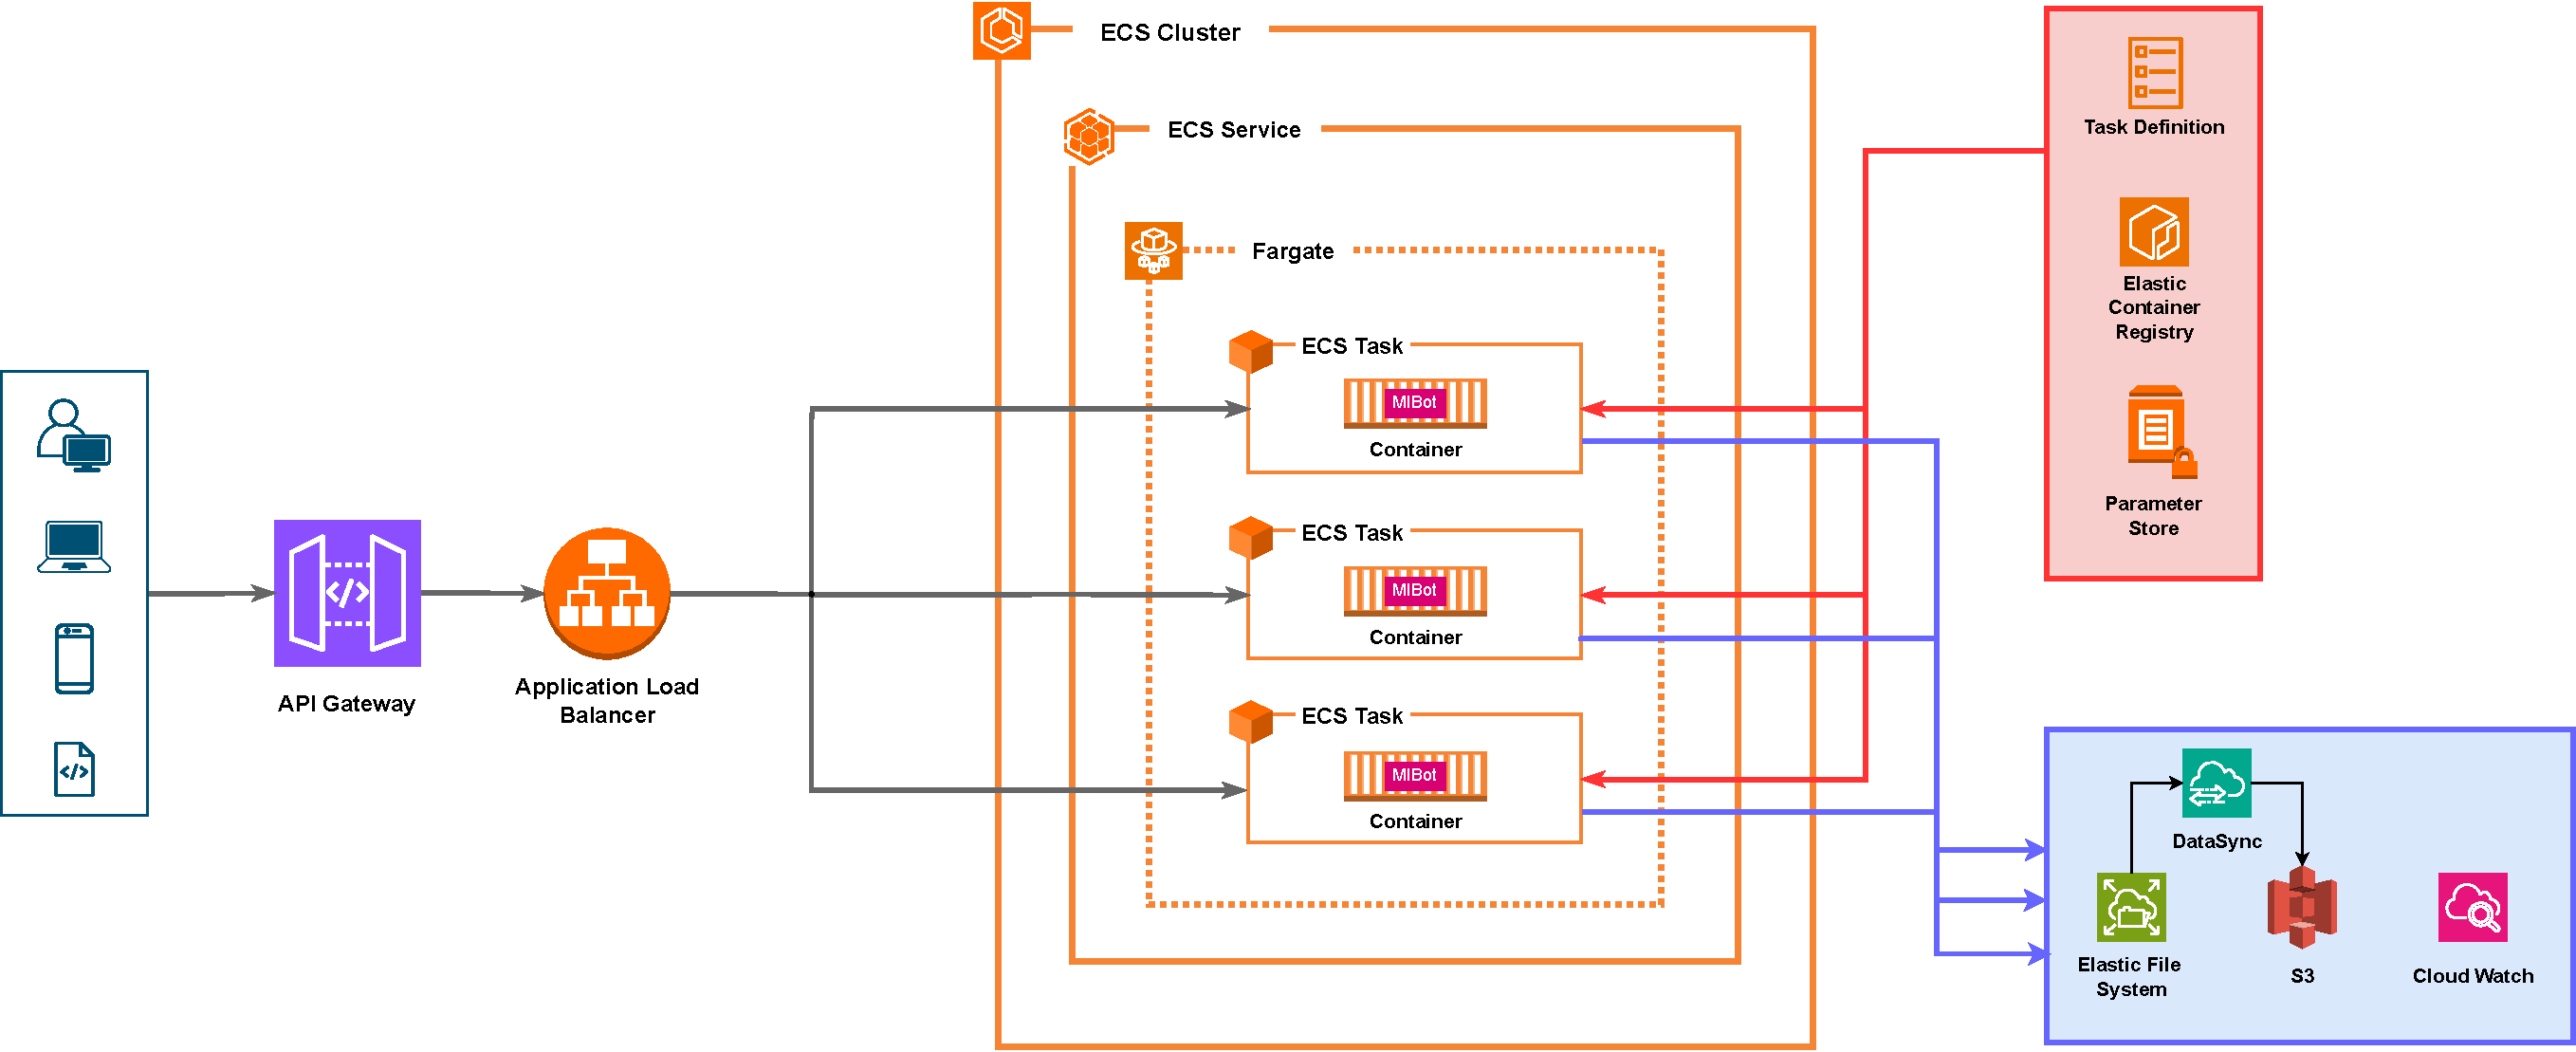
\includegraphics[width=0.99\linewidth]{fig/deployment.drawio.pdf} 
  \caption{Containerized MIBot application deployed to ECS.}
  \label{fig:ecs-components}
\end{figure}

\paragraph{1. ECS Cluster:}To deploy MIBot to ECS, we first provisioned an \textbf{ECS cluster} (\texttt{mibot-v6-cluster}). An ECS cluster is a \textit{logical} grouping of heterogeneous compute resources. To understand what we mean by this, let's first see what a compute resource is in the context of AWS. An AWS \textbf{compute resource} is any AWS-managed infrastructure component that provides processing power for running applications or workloads. Examples include Elastic Cloud Compute (EC2), AWS Lambda, AWS Fargate, etc. Some of the compute resources are \textbf{user-managed}, like EC2, where users rent virtual machines to run and manage their applications. In contrast, AWS Fargate is \textbf{fully managed} and is used to run containerized applications. A cluster is merely a logical grouping of such compute resources.

In our ECS cluster, however, we only used \textbf{AWS Fargate} as the computing resource. Apart from the ability to deploy the containerized MIBot application without having to manage our own servers, AWS Fargate also provided us with \emph{spot runs} for cost optimization. In the \texttt{FARGATE\_SPOT} mode, tasks run on spare compute capacity. If a container receives no traffic in the last two hours and AWS needs the capacity back, the task will be terminated. ECS will detect this event and will almost immediately instantiate a new task for the application.

\paragraph{2. ECS Service:}Inside the ECS cluster, we created an \textbf{ECS Service} (\texttt{mibot-v6-service}). The ECS Service contains the deployment configuration of the application. For example, the number of desired replicas of the application (also called \emph{tasks}) that should run at any given time.  For our study, we set this to use two tasks. If one of the tasks fails for some reason, the ECS Service replaces it automatically. It can also be configured to increase the number of tasks when it detects higher-than-normal traffic. The Service is connected to an Elastic Load Balancer (ELB) to distribute incoming traffic evenly among tasks. Most importantly, it also defines deployment (rolling update, blue/green deployment) and rollback strategies. It can leverage the AWS circuit breaker to roll back failed deployments automatically.

\paragraph{3. ECS Task Definition:}The final piece in MIBot's deployment is defining a \textbf{Task}. A \texttt{Task} runs a specific container after downloading it from the Elastic Container Registry (ECR). The \texttt{Task} definition specifies environment variables and API credentials that are securely stored in AWS Systems Manager Parameter Store and are injected into the container (e.g., \texttt{OPENAI\_API\_KEY}) when the task is started. It further defines a \emph{health check} for the container. The health check sends a request to the \texttt{/health} endpoint on the container's port~80 every five minutes. If the response is anything other than \texttt{OK 200} or it does not get a response within one minute, it deems the container unhealthy. The \texttt{Service} terminates the \texttt{Task} and replaces it with a new one. The task definition further contains required CPU and memory (1024 mcpu and 4~GB, respectively, in the case of MIBot). The containers also mount a persistent Amazon Elastic File System (EFS) volume to store conversation transcripts and evaluation metrics. Furthermore, all container logs are written in AWS CloudWatch for retrospective analysis of the system's behaviour.

\subsection{Other Components of the Deployment}

\paragraph{Load Balancer:}We configured an Elastic Load Balancer (\texttt{mibot-elb}) with three subnets for high availability, meaning we have three instances of load balancers in three different Availability Zones. The load balancers are the modern \emph{application} load balancers (ALB), which are internet-facing and associated with a security group permitting inbound traffic on port 443. The DNS names allow external users to connect to the service through a friendly domain. The ALB routes incoming HTTP requests to the ECS service's target group and internal health check requests to the \texttt{/health} endpoint.

\paragraph{API Gateway:}We also provisioned an AWS API Gateway, which acts as a reverse proxy and enables secure TLS termination and request throttling. The gateway exposes HTTPS endpoints for \texttt{/chat}, \texttt{/get\_transcript}, \texttt{/health}, \texttt{/info}, and \texttt{/s3\_upload}. Each path includes \texttt{OPTIONS} methods to enable cross-origin requests and defines the expected response headers. This allows client browsers (running the frontend code) to send requests to MIBot without getting a ``Cross-Origin Request Blocked'' error or ``Not Secure'' warning.

\paragraph{DataSync:}Conversation transcripts and metadata are stored on both an encrypted EFS volume and AWS S3 only when the participant clicks on the final Submit button at the end of the study session. EFS acts as a redundant data layer in case the upload to S3 fails for some reason. For eventual consistency, we periodically copy files from EFS to S3 with the help of AWS DataSync, which runs a daily CRON job.

\subsection{Deployment Pipeline}
We adopted automated development practices for deployment. Every time we push a special `\texttt{production}' Git tag to the remote main branch, a GitHub Workflow builds the Docker image, runs unit tests, and, if tests pass, pushes the image to Amazon ECR. Another workflow triggers a CloudFormation deployment that updates the ECS task definition with the new image tag and performs a rolling deployment of the ECS Service. Deployment uses a circuit breaker configuration: if the service fails health checks, the rollout is automatically rolled back to the previous stable revision. By integrating the deployment pipeline into version control, we ensured automated deployments tied to code changes.


\section{Feasibility Study with Human Smokers}
\label{sec:feasibility}
The deployed MIBot system was used in a \margindex{Feasibility Study}feasibility study with human smokers. The goal of the study was to determine the impact of a single-session interaction with MIBot and assess its safety for delivery to ambivalent smokers in a real-world setting.

\subsection{Ethics Approval and Consent}
The protocol was approved by the \margindex[Feasibility Study]{ethics approval}University of Toronto Research Ethics Board under protocol number 49997 (approved August~3, 2024) and adhered to all institutional guidelines. Before participating in the study, prospective participants reviewed an online consent form that outlined study aims, procedures, compensation, potential risks, and data handling practices. Participation required explicit electronic consent. Risks were described as minimal but included the possibility that discussing smoking could cause stress or temporarily increase cravings. No personally identifying information was collected, and all data were de-identified prior to release.

\subsection{Participant Recruitment}
\label{sec:recruitment}
\margindex[Feasibility Study]{participant recruitment}[Recruitment]Participants were recruited via \margindex[Feasibility Study, Recruitment]{prolific}\textit{Prolific}\footnote{\url{https://www.prolific.com}}, an online behavioural research platform with pre-screened participant pools and built-in demographic filters. Prolific was chosen for its ability to target recruitment to specific smoking status, demographic characteristics, and quality-control thresholds, and for its established use in prior MI chatbot studies~\citep{brown2023motivational,info:doi/10.2196/20251}. Participants received \pounds5.50 for the main session and \pounds1.00 for the follow-up survey, exceeding Prolific's recommended hourly rates.


\subsubsection{Initial Screening Criteria}
\margindex[Feasibility Study, Recruitment]{screening criteria}[Screening]Eligibility screening was implemented at two levels: (1) \textit{Prolific} prescreen filters, applied before invitation to the study; and (2) an \margindex[Feasibility Study, Recruitment]{in-study screening}[In-Study Screen]in-study screening step prior to chatbot interaction. The first set of filters required that all invitees be 18 years or older, be fluent in English, have an approval rate of at least 90\% on prior Prolific studies and self-identify as a \emph{current smoker} of at least five cigarettes per day, with a history of smoking at this rate for one year or more.

In addition, recruitment was set up to aim for a nearly equal sex balance. Although the final sample reflected slight deviations due to subsequent exclusion filtering, this pre-allocation ensured coverage across male and female participants.

\subsubsection{In-Study Screening}

\noindent Baseline demographics of enrolled participants are summarized in Table~\ref{tab:participant-characteristics}. All were English-speaking adults who self-identified as current daily smokers and passed prescreening and in-study eligibility checks on Prolific. The sample was approximately sex-balanced with broad age coverage. Residence was primarily the United Kingdom and United States, with additional participants from Canada and South Africa. Unless otherwise specified, values are presented as counts (n) and percentages (%). Age is reported as median, mean (SD), and range.

\subsubsection{Participant Characteristics}
\label{subsec:participant-characteristics}
\begin{table}[htbp]
\centering
\caption{Baseline characteristics of enrolled participants}
\begin{tabular}{l l}
\hline
\textbf{Characteristic} & \textbf{n (\%)} \\
\hline
Total participants & 106 \\
\hline
Sex & \\
\quad Female & 57 (53.8) \\
\quad Male & 49 (46.2) \\
\hline
Language & \\
\quad English-speaking & 106 \\
\hline
Age summary & Range 22--77; median 38; mean 40 (SD 13) \\
Age groups (years) & \\
\quad Below 20 & 0 (0.0) \\
\quad 20 to 29 & 26 (24.5) \\
\quad 30 to 39 & 32 (30.2) \\
\quad 40 to 49 & 20 (18.9) \\
\quad 50 to 59 & 19 (17.9) \\
\quad 60 to 69 & 6 (5.7) \\
\quad 70 to 79 & 3 (2.8) \\
\quad Above 79 & 0 (0.0) \\
\hline
Ethnicity & \\
\quad White & 80 (75.5) \\
\quad Black & 9 (8.5) \\
\quad Asian & 7 (6.6) \\
\quad Mixed & 5 (4.7) \\
\quad Other & 5 (4.7) \\
\hline
Student status & \\
\quad No & 80 (75.5) \\
\quad Yes & 21 (19.8) \\
\quad Data expired & 5 (4.7) \\
\hline
Employment status & \\
\quad Full-time & 49 (46.2) \\
\quad Part-time & 18 (17.0) \\
\quad Not in paid work & 16 (15.1) \\
\quad Unemployed & 13 (12.3) \\
\quad Other & 10 (9.4) \\
\hline
Country of residence & \\
\quad United Kingdom & 47 (44.3) \\
\quad United States & 42 (39.6) \\
\quad Canada & 9 (8.5) \\
\quad South Africa & 4 (3.8) \\
\quad Other & 4 (3.8) \\
\hline
Country of birth & \\
\quad United Kingdom & 44 (41.5) \\
\quad United States & 39 (36.8) \\
\quad Canada & 6 (5.7) \\
\quad Kenya & 3 (2.8) \\
\quad South Africa & 3 (2.8) \\
\quad Germany & 2 (1.9) \\
\quad Other & 9 (8.5) \\
\hline
\end{tabular}
\label{tab:participant-characteristics}
\end{table}


Upon accessing the study website, participants completed a smoking status confirmation question identical to Prolific's prescreen question. From an initial pool of 159 participants, we screened for ambivalence using the \textit{Readiness Ruler}, as described in Section~\ref{subsec:readiness-ruler}. To ensure participants were in a state where MI could be beneficial, we included those with a pre-conversation \emph{confidence-to-quit} score of 5 or less on a 10-point scale. We also included 'discordant'
participants, who, despite having high confidence (a score greater than 5), rated the importance of quitting at least five points lower than their confidence. This process resulted in a final sample of 106 participants.


Participants who met all criteria and provided informed consent proceeded to the survey phase. Those who did not meet the eligibility criteria were redirected to the Prolific platform without completing the study.

\subsection{Study Procedure}
\begin{figure}[ht]
    \centering
    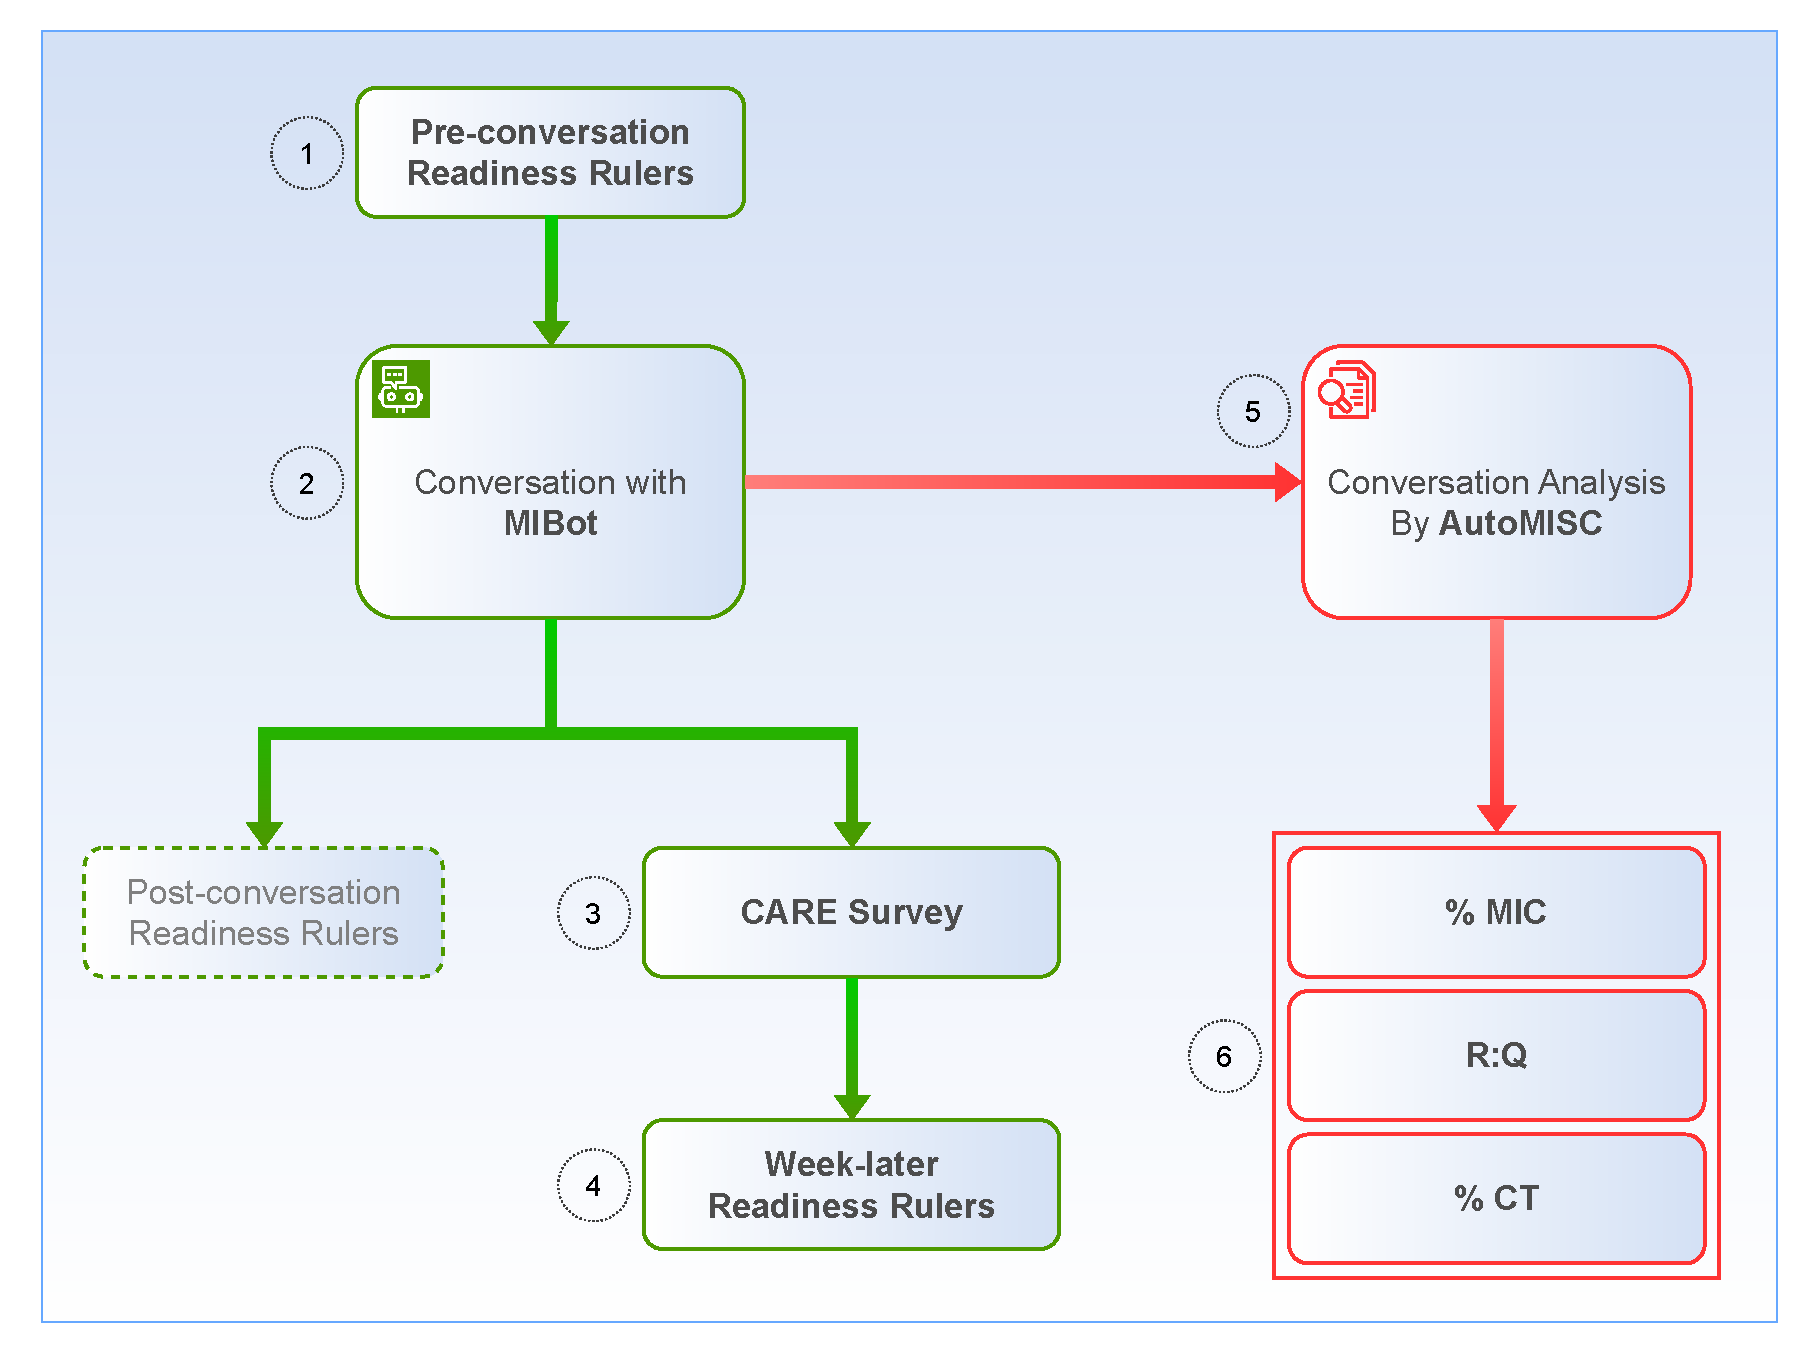
\includegraphics[width=0.9\linewidth]{fig/feasibility_study_flow.pdf}
    \caption{Overview of the feasibility study protocol.}
    \label{fig:study-flow}
\end{figure}

The full \margindex[Feasibility Study]{study procedure}study procedure comprised four major phases: (1) \margindex[Feasibility Study, Procedure]{pre-conversation surveys}[Pre-Surveys]pre-conversation surveys; (2) a single text-based conversation with MIBot; (3) \margindex[Feasibility Study, Procedure]{post-conversation surveys}[Post-Surveys]immediate post-conversation surveys; and (4) a \margindex[Feasibility Study, Procedure]{one-week follow-up}[Follow-Up]one-week follow-up survey. Figure~\ref{fig:study-flow} illustrates the progression.



\paragraph{Phase 1: Pre-Conversation Surveys:}
Before interaction with MIBot, participants completed:
\begin{enumerate}
    \item \textbf{\margindex[Feasibility Study, Surveys]{heaviness of smoking index (HSI)}[HSI]Heaviness of Smoking Index (HSI)}~\citep{heatherton1989measuring} survey, which assesses nicotine dependence via two questions:
        \begin{enumerate}
            \item number of cigarettes smoked per day (scored 0-3), and
            \item time to first cigarette after waking (scored 0-3).
        \end{enumerate}
    The HSI score is the sum of these two items, and ranges from 0 to 6, with higher scores indicating greater nicotine dependence.
    \item \textbf{Quit Attempts in the Past Week}: number of conscious attempts to abstain from smoking for at least 24 hours during the preceding seven days.
    \item \textbf{Readiness Ruler}: three questions measuring self-reported ratings of importance, confidence, and readiness to quit on 0–10 scales (Section~\ref{subsec:readiness-ruler}).
\end{enumerate}

\paragraph{Phase 2: Conversation with MIBot:}
Participants engaged in a single MI-style conversation via a web-based text interface.

\paragraph{Phase 3: Post-Conversation Surveys:}
Immediately after the conversation, participants repeated the Readiness Ruler, completed the CARE empathy scale (Section~\ref{subsec:care}), and provided qualitative feedback on the chatbot's performance.

\paragraph{Phase 4: One-Week Follow-Up:}
Seven days later, participants were invited via Prolific to complete a follow-up survey. This included a third administration of the Readiness Ruler and questions about quit attempts and changes in smoking behaviour over the past week.

\subsection{Survey Instruments}
\label{subsec:survey-instruments}

The goal of the work is to move ambivalent smokers towards the decision to quit. We employed the following metrics to measure outcomes from the interaction. In addition to the primary outcome measures, we also recorded other survey instruments to get a holistic picture of the chatbot's effectiveness.

\subsubsection{1. Readiness Ruler}
\label{subsec:readiness-ruler}
The Readiness Ruler~\citep{rollnick1992development} is a validated tool for assessing motivational state across three dimensions:
\begin{itemize}
    \item \textbf{Importance:} ``How important is it to you right now to stop smoking?''
    \item \textbf{Confidence:} ``How confident are you that you would succeed at stopping smoking if you started now?''
    \item \textbf{Readiness:} ``How ready are you to start making a change at stopping smoking right now?''
\end{itemize}
Responses were recorded on an 11-point scale (0 = ``not at all'', 10 = ``extremely''). The week-later change in \emph{confidence} from the pre-conversation value was used as the primary metric for the chatbot's effectiveness, as this is the most predictive
of downstream quitting success~\cite{Gwaltney2009-wj,Abar2013}.

\subsubsection{2. CARE Measure}
\label{subsec:care}
The \margindex[Feasibility Study, Surveys]{care measure}[CARE]Consultation and Relational Empathy (CARE) measure~\citep{mercer2004consultation,bikker2015measuring} assesses perceived empathy in clinical encounters. Ten items evaluate the counsellor's ability to make the participant feel at ease, listen actively, appreciate the participant as a whole person, and collaborate on problem-solving. Each question is rated on a 0-5 scale, with a total score range of 0-50.

\subsubsection{3. Qualitative Feedback}
Three open-ended questions solicited \margindex[Feasibility Study, Surveys]{qualitative feedback}subjective impressions:
\begin{enumerate}
    \item ``What are three words that you would use to describe the chatbot?''
    \item ``What would you change about the conversation?''
    \item ``Did the conversation help you realize anything about your smoking behaviour? Why or why not?''
\end{enumerate}
These responses can inform future prompt refinements and provide contextual data for interpreting quantitative outcomes.

\subsubsection{4. Follow-Up Quit Attempt Survey}
At one week, participants reported whether they had made any quit attempts in the preceding seven days, the number of attempts, and whether any changes in smoking habits had occurred. This included partial changes such as a reduction in cigarettes per day.

\subsection{Automated Conversation Analysis}
\label{subsec:automisc}
In addition to participant-reported outcomes, conversations were analyzed for MI adherence and elicitation of motivational language using \textit{AutoMISC}, an automated implementation of the Motivational Interviewing Skill Code v2.5~\citep{Houck2010}. The AutoMISC system was primarily developed by Soliman, as described in his thesis [CITE\_THESIS], with further validation in~\cite{ali2025automated}. For this project, we utilized the existing AutoMISC system and contributed to the work described in~\cite{mahmood-etal-2025-fully}. The analysis pipeline first segments each conversational volley into individual utterances. Then, it classifies counsellor utterances as MI-Consistent, MI-Inconsistent, Reflection, Question, or Other. Similarly, it classifies each client utterance as exhibiting Change Talk, Sustain Talk, or Neutral. Finally, it computes the following: \%~MI-Consistent Responses (\%MIC), Reflection-to-Question Ratio (R:Q), \%~Client Change Talk (\%CT). AutoMISC was validated against human coders, including two MI-expert clinicians \cite{mahmood-etal-2025-fully}.


Readiness rulers (especially the week-later change in \emph{confidence}), CARE, and AutoMISC summary metrics together provide a holistic view of the MIBot intervention, assessing its effectiveness, perceived empathy, safety, and adherence to MI principles. In the next chapter, we report the results from our human feasibility study on these metrics.

